\documentclass{article}
\usepackage{PRIMEarxiv}
\usepackage[utf8]{inputenc} % allow utf-8 input
\usepackage[T1]{fontenc}    % use 8-bit T1 fonts
\usepackage{palatino,eulervm}
\usepackage{hyperref}       % hyperlinks
\usepackage{url}            % simple URL typesetting
\usepackage{booktabs}       % professional-quality tables
\usepackage{amsfonts}       % blackboard math symbols
\usepackage{nicefrac}       % compact symbols for 1/2, etc.
\usepackage{microtype}      % microtypography
\usepackage{lipsum}
\usepackage{fancyhdr}       % header
\usepackage{graphicx}       % graphics
\graphicspath{{media/}}     % organize your images and other figures under media/ folder
\usepackage{minted}

\pagestyle{fancy}
\thispagestyle{empty}
\rhead{ \textit{ }} 

\fancyhead[LO]{SVD Factorization for Tall-and-Fat Matrices on Paralel Architectures}
  
\title{SVD Factorization for Tall-and-Fat Matrices on Paralel Architectures}

\author{
  Burak Bayramlı \\
  İstanbul, Turkey\\
  \texttt{burakbayramli.github.io} 
}


\begin{document}

\maketitle

\begin{abstract}
We demonstrate an implementation for an approximate rank-k SVD factorization,
combining well-known randomized projection techniques with previously known
paralel solutions in order to compute steps of the random projection based SVD
procedure. We structure the problem in a way that it reduces to fast computation
around $k \times k$ matrices computed on a single machine, greatly easing the
computability of the problem. The paper is also a tutorial on paralel linear
algebra methods using a plain architecture without burdensome frameworks.
\end{abstract}


% keywords can be removed
\keywords{Parallel \and Concurrency \and Big Data}

\section{Introduction}


Multiplication

\begin{verbatim}
for(int m = 0; m < M; m++) {
    for(int k = 0; k < K; k++) {
        for(int n = 0; n < N; n++) {
            C[m][n] += A[m][k]*B[k][n];
        }
    }
}
\end{verbatim}

\begin{figure}[h]
  \centering
  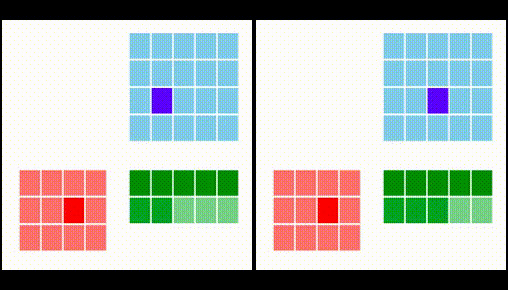
\includegraphics[width=20em]{mult1.jpg}
  \caption{Two Steps of a Row Based Multiplication Process}
  \label{fig:mult1}
\end{figure}


SVD

$$
A^TA = V \Sigma^2 V^T 
$$

$$
A = U \Sigma V^T \to U = A V \Sigma^{-1}
$$

\section{Implementation}

Big Data became possible largely thanks to Map/Reduce architectures which
represent splitting (mapping) and grouping (reducing) concepts logically and
present them the only interface for a programmer to worry about, while in the
background directing data pieces produced by mapping and reducing to appropiate
seperate nodes to achieve concurrency. A sample process is seen in
Figure~\ref{fig:mapreduce1},

\begin{figure}[h]
  \centering
  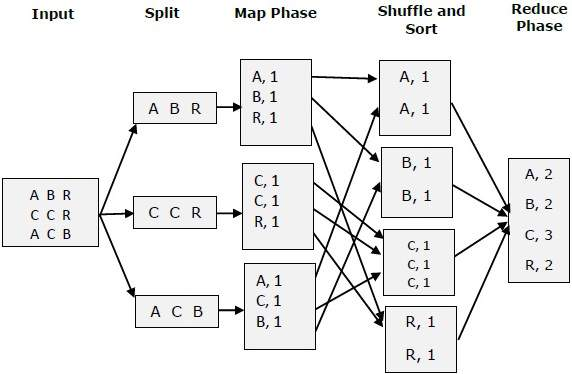
\includegraphics[width=20em]{mapreduce1.jpg}
  \caption{Example of Map Reduce}
  \label{fig:mapreduce1}
\end{figure}

\begin{figure}[h]
  \centering
  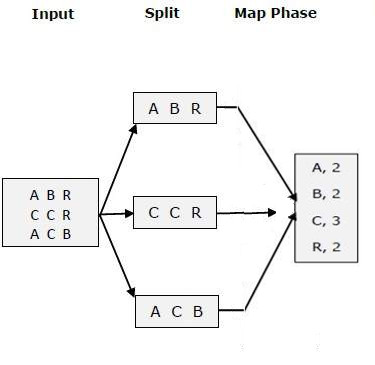
\includegraphics[width=15em]{splitprocess.jpg}
  \caption{Split Process}
  \label{fig:mapreduce1}
\end{figure}

\subsection{Architecture}

\begin{minted}[fontsize=\footnotesize]{python}
import os, numpy as np

def process(file_name,N,hookobj):
    file_size = os.path.getsize(file_name)
    beg = 0
    chunks = []
    for i in range(N):
        with open(file_name, 'r') as f:
            s = int((file_size / N)*(i+1))
            f.seek(s)
            f.readline()
            end_chunk = f.tell()-1
            chunks.append([beg,end_chunk])
            f.close()
        beg = end_chunk+1
    c = chunks[hookobj.ci]
    with open(file_name, 'r') as f:
        f.seek(c[0])
        while True:
            line = f.readline()
            hookobj.exec(line)
            if f.tell() > c[1]: break
        f.close()
        hookobj.post()
\end{minted}

\subsection{Calcuation of $A^T A$}

\begin{minted}[fontsize=\footnotesize]{python}
class ATAJob:
    def __init__(self,D,ci):
        self.C = np.zeros((D,D))
        self.ci = ci
    def exec(self,line):
        tok = line.split(';')
        vec = np.array([float(x) for x in tok])
        self.C = self.C + np.outer(vec, vec)
    def post(self):
        outfile = "/tmp/C-%d.csv" % self.ci
        np.savetxt(outfile, self.C, delimiter=';',fmt='%1.6f')
\end{minted}

\subsection{$A$ Multiplication}

\begin{minted}[fontsize=\footnotesize]{python}
class MultJob:
    def __init__(self,ci,bfile):
        self.afile = ""
        self.B = np.loadtxt(bfile,delimiter=';')
        self.ci = ci
        cname = "%s/C-%d.csv" % (os.path.dirname(afile), self.ci)
        self.outfile = open(cname, "w")        
    def exec(self,line):        
        vec = np.array([np.float(x) for x in line.strip().split(";")])
        vec = np.reshape(vec, (len(vec),1))
        res = (vec * self.B).sum(axis=0).tolist()  
        res = ";".join(map(str, res))
        self.outfile.write(res)
        self.outfile.write("\n")
        self.outfile.flush()
    def post(self):
        self.outfile.close()
\end{minted}



%Bibliography
\bibliographystyle{unsrt}  

\begin{thebibliography}{1}

\bibitem{gleich}
Gleich, Benson, Demmel, \emph{Direct QR factorizations for tall-and-skinny
  matrices in MapReduce architectures}, {\tt arXiv:1301.1071 [cs.DC]}, 2013

\bibitem{halko}
N.~Halko, \emph{Randomized methods for computing low-rank approximations of
  matrices}, University of Colorado, Boulder, 2010

\bibitem{gupta}
S.~Dangupta, A.~Gupta \emph{An Elementary Proof of a Theorem of Johnson and
  Lindenstrauss}, Wiley Periodicals, 2002

\bibitem{kurucz}
M.~Kurucz, A. A.~Benczúr, K.~Csalogány, \emph{Methods for large scale SVD with
missing values}, ACM, 2007

\bibitem{zadeh}
Zadeh, \emph{CME 323: Distributed Algorithms and Optimization, Lecture 17}, 
\url{https://stanford.edu/~rezab/classes/cme323/S17/}

\bibitem{agrawal}
Agrawal, \emph{Matrix Multiplication: Inner Product, Outer Product and Systolic Array},
\url{https://www.adityaagrawal.net/blog/architecture/matrix_multiplication}
  
\end{thebibliography}

\end{document}
